
\section{3D Displays}
\subsection{Two-view 3D displays}
\begin{frame}

  \frametitle{3D Displays \\Two-view 3D displays} 
  
  \begin{itemize}
  \item Wavelength Selective Displays:
    
    \begin{itemize}
    \item Each eye receives the image intended for it
    \item Images are filtered	
    \end{itemize}
    
    
    
  \item Advantage:
    \begin{itemize} 	
    \item Any color display device can be used to present the stereoscopic
    \end{itemize}
    \end{itemize}
  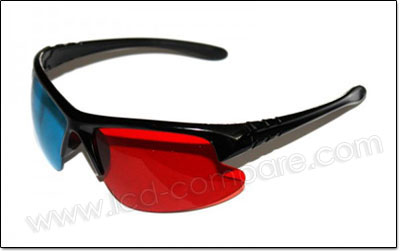
\includegraphics[keepaspectratio,height=.13\linewidth]{1.jpg}
\end{frame}


\begin{frame}		  	
  \begin{itemize}
  \item Time-Sequential Two-View Displays:
    \begin{itemize}
    \item Time-Sequential Polarization:
      \begin{itemize}
      \item Pair of passive polarizing glasses
      \item Each lens is polarized in one direction
      \item The image displayed on the screen is actually composed of two images
      \end{itemize}
    \end{itemize}
  \end{itemize}
  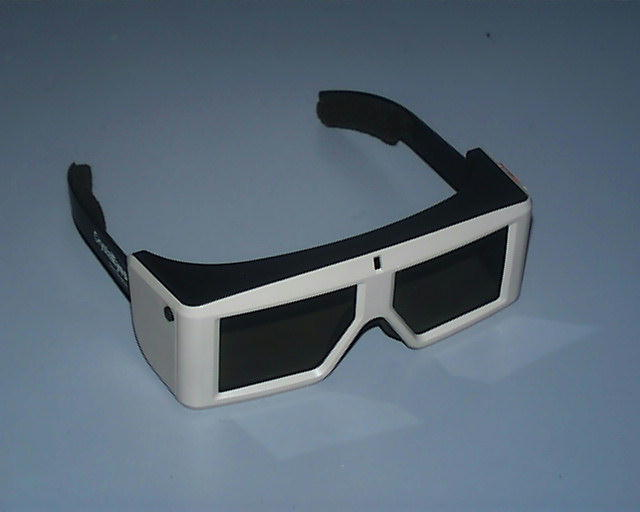
\includegraphics[keepaspectratio,height=.2\linewidth]{2.jpg}
\end{frame}

\subsection{Horizontal parallax multiview 3D displays}	

\begin{frame}

  \frametitle{Écrans 3D \\Horizontal parallax multiview 3D displays} 
  
  \begin{itemize}
  \item Parallax Barrier Displays:
    
    \begin{itemize}
    \item This is an autostereoscopic technical.
    \item It provides a terrain vision without wearing glasses.
    \end{itemize}
  \item the disadvantages:
    \begin{itemize} 	
    \item	It must be placed precisely in relation to the screen.
    \item Must be stable.
    \item It does not allow viewing of the stereoscopic image at the same time several viewers.
    \end{itemize}
  \end{itemize}
  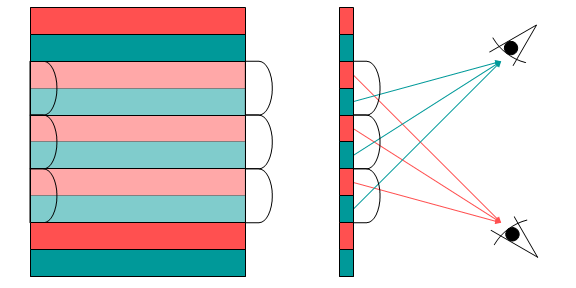
\includegraphics[keepaspectratio,height=.13\linewidth]{4.png}
\end{frame}

\begin{frame}
  \begin{itemize}
  \item Multi-Projector Displays:\\
 This technique involves a position in a circle several video projectors displaying all an angle different image after these images are projected on a special screen.			
  \item Advantage:
    \begin{itemize} 
    \item Size of the 3D image can be much larger it is no limit.
    \end{itemize}
  \item the disadvantages:
    \begin{itemize} 	
    \item	Multiple projectors are needed (projector view)
    \item Headlamps must be accurately aligned.
    \end{itemize}
  \end{itemize}
\end{frame}

\subsection{Full parallax multiview 3D displays} 
\begin{frame}
  \frametitle{Écrans 3D \\Full parallax multiview 3D displays} 
  
This type of display allows viewers to view a 3D scene from any angle.\\
  
  \begin{itemize}
  \item Integral Imaging Displays:
    
    \begin{itemize}
    \item It is a way of auto-stereoscopic 3D display, which was originally proposed by Lippmann in 1908.

    \item This technical consists in using a network of micro-lenses in front of each image.

    \end{itemize}
  \end{itemize}
  
\end{frame}
\begin{frame}
  \frametitle{Analyse} 
  
  \begin{itemize}
  \item For a 3D display:
    \begin{itemize}
    \item Eye position
    \item Constraints on the position of the head
    \end{itemize}
  \end{itemize}

  \begin{itemize}
  \item Application:
    \begin{itemize}
    \item cinema
    \item reporting and advertising
    \item 3D for mobile devices
    \end{itemize}
  \end{itemize}
  \begin{itemize}
  \item The Stereoscopic  and auto-stereoscopic technologies
  \item holography
  \end{itemize}
\end{frame}


